\section{EnsembleVis}
\label{sec:EnsembleVis}

This section presents the experience behind our fully virtual collaboration between researchers from multiple UK institutions, chronicling the development of EnsembleVis.

% Change to paragraphs

\subsection{First Meeting - 27 July 2020}
\label{subsec:InitialMeeting}
On 27 July 2020, amid the UK's first national lockdown and stricter measures imposed by local authorities, we convened the initial virtual meeting with VIS researchers from King's College London, Loughborough University, Swansea University, University of Nottingham, University of Warwick, and University of Oxford.

During the meeting, we received an overview of the SCRC and the responsibilities of the visualization volunteer team.
Our assigned task was to create visualizations for the model, with the purpose of allowing the modellers to analyze the outcomes of the model.

Following the initial meeting, we engaged in email correspondence with the modellers to delve into the visualization requirements. The modellers shared a comprehensive list of parameters and model outcomes, along with the corresponding outcome data.
\subsection{First Commit - 14 Sep 2020}
We proceeded to create an initial prototype of the visualization, which was subsequently reviewed by the modellers.
Incorporating their input, we refined the prototype during our weekly internal discussions.
On 14 Sep 2020, England introduced the 'rule of six', which banned any gatherings above six.
On the same day, we made our first commit to a GitHub repository, signifying the commencement of our development.
At the same time, we began preprocessing the data.

A week after the initial commit, the UK witnessed the implementation of additional restrictions, such as mandatory work from home and a 10pm curfew.

\subsection{First Visualization, Second Meeting - 5 Nov 2020}
On 5 Nov 2020, the first day of the second national lockdown in the UK, we completed the first visualization, a parallel coordinates plot, see \Cref{fig:1st-vis}.
This followed by the second meeting with VIS researchers from other institutions, where we received feedback on the visualization, on 6 Nov 2020.
\begin{figure}
    \centering
    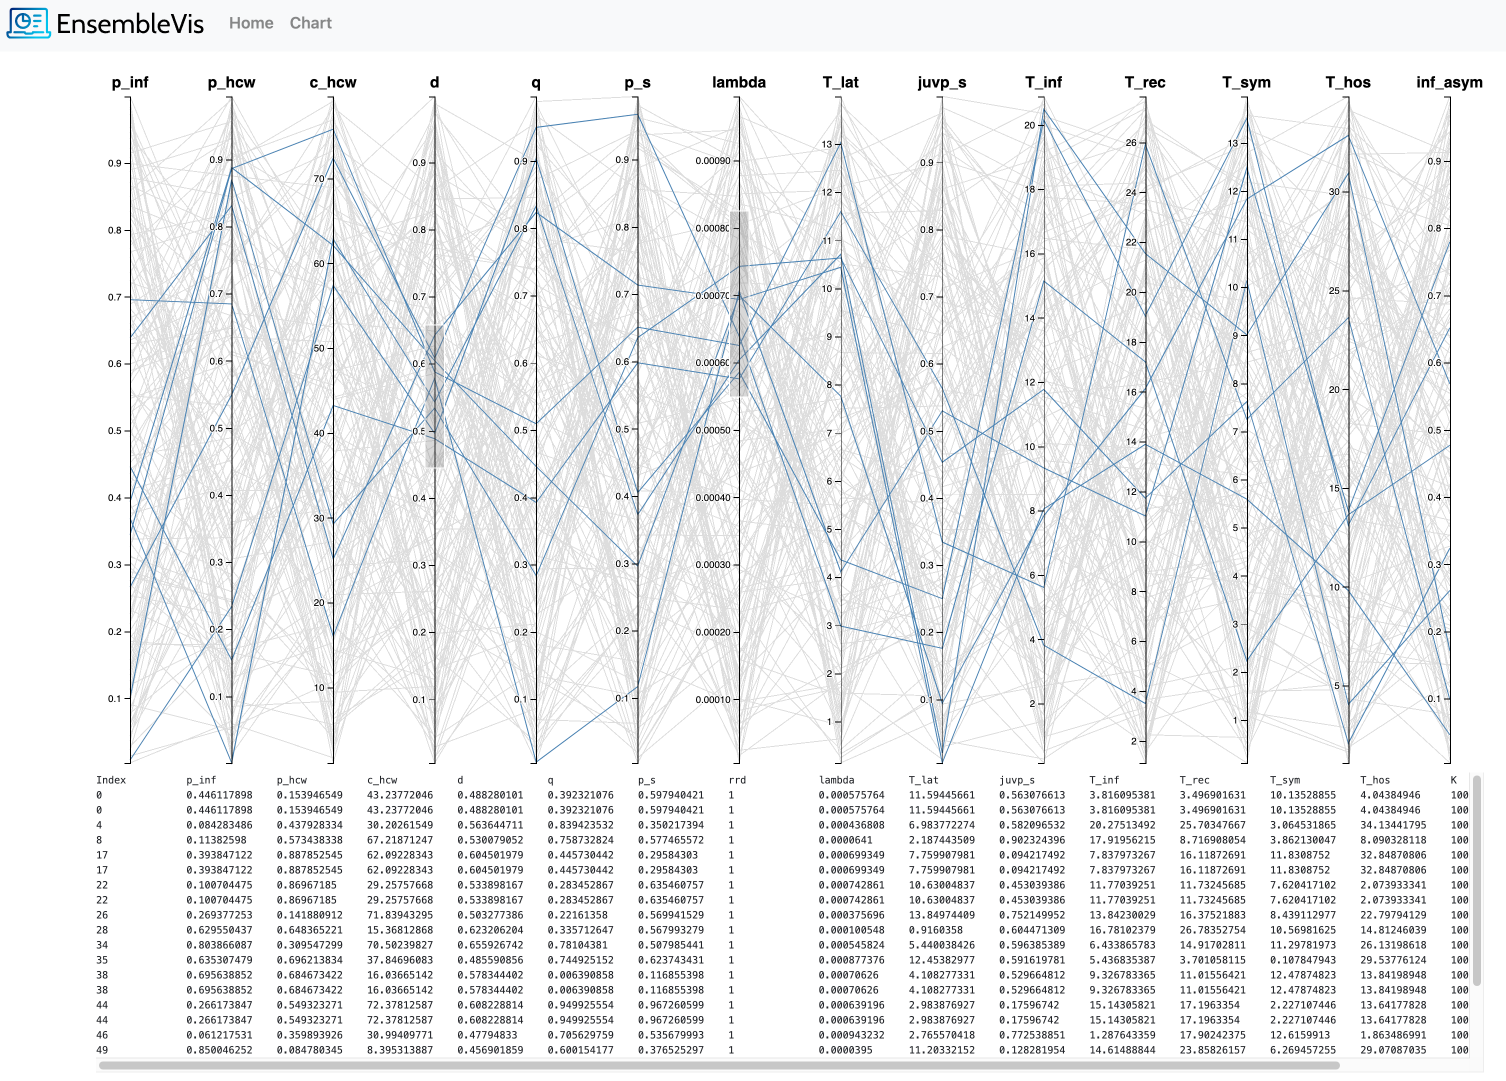
\includegraphics[width=\linewidth]{1st-vis.png}
    \caption{The first visualization, a parallel coordinates plot visualizing all 160 configurations of the model, was completed on 5 Nov 2020. This visualization was developed utilizing D3.js and incorporated a brushing feature, enabling users to filter the configurations.
    }
    \label{fig:1st-vis}

\end{figure}

\subsection{Third Meeting - 11 Nov 2020}
On 11 Nov 2020, the group convened for the third meeting, where we received further feedback on the visualization. As per the modellers' requests conveyed through emails, we incorporated a line chart to depict the model outcomes, see \Cref{fig:1st-line}.

\begin{figure}
    \centering
    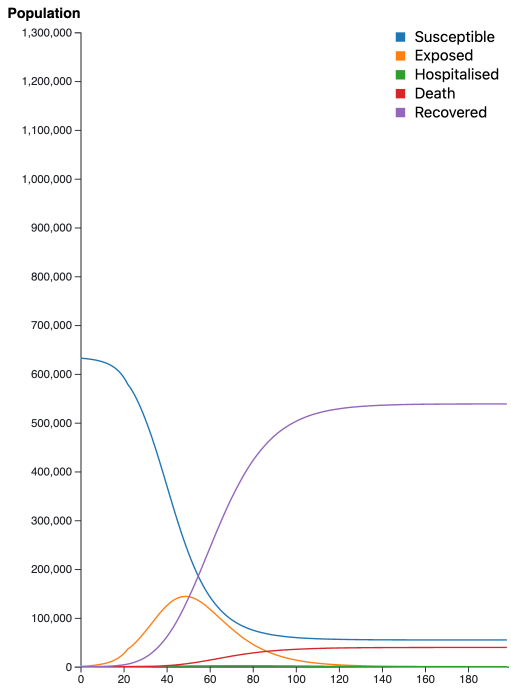
\includegraphics[width=\linewidth]{1st-line.png}
    \caption{A line chart was added to the visualization on 11 Nov 2020, to visualize the model outcomes.
    The x-axis of the chart corresponds to the number of days since the first available date in the Scottish dataset (specific date unknown to us), while the y-axis represents the population.
    To differentiate between different population categories, a color map was employed: susceptible (blue), exposed (orange), death (red), hospitalized (green), and recovered (purple).
    The final version of this chart which includes all the simulation results, is shown in \Cref{fig:teaser}D.
    }
    \label{fig:1st-line}

\end{figure}

\subsection{Fourth Meeting - 25 Nov 2020}
On 25 Nov 2020, the group convened for the fourth meeting, held just a day after the announcement of the gathering rules for Christmas in the UK.
During the meeting, we received feedback on the new visualization, a table with glyphs, see \Cref{fig:teaser}B. We incorporated this table view featuring glyphs to visualize all 160 input parameter configurations, following discussions with the modellers.
Each parameter is symbolized by a glyph, with the color of the glyph corresponding to its deviation from the average value.
The view provides the functionality to sort the parameters according to their values and can be dynamically updated by brushing the parallel coordinates plot for the input parameters (\Cref{fig:teaser}A).

\subsection{Fifth Meeting - 9 Dec 2020}
On 9 Dec 2020, a week after the end of the second national lockdown in the UK, with England facing a stricter three-tier restriction policy, the group convened for the fifth meeting.
At this point, we still had not met with the modellers, all communications and discussions took place through emails.

\subsection{Sixth Meeting - 10 Dec 2020}
On 10 Dec 2020, we finally met with modelers from the University of Edinburgh, the University of Exeter, the University of Glasgow, The London School of Hygiene \& Tropical Medicine, for the first time.
In contrast to sharing screenshots via email and deploying a website with a live view of our development (which they might not have been proficient in using), we delivered a live presentation, fielding numerous questions.
The modellers were extremely pleased with the visualization, and a list of feedback was provided:
\begin{enumerate}
    \item The modellers found the parallel coordinates plot very useful, and requested the incorporation of another one for the model outcomes. We implemented this as shown in \Cref{fig:teaser}C.
    \item The modellers requested all the simulation results to be displayed in \Cref{fig:1st-line}, with the current one being highlighted. We implemented this as shown in \Cref{fig:teaser}D.
    \item The modellers requested the incorporation of a scatterplot to visualize the model outcomes, specifically, a Principal Component Analysis (PCA) result obtained from other volunteers. We implemented this as shown in \Cref{fig:teaser}E.
\end{enumerate}

Furthermore, we received the exciting news that funding had been successfully secured, leading to the transition of our volunteer work to a team of paid developers, who would continue with further development of the project on a future date.

\subsection{Last Commit - 28 Apr 2021}
By 28 Apr 2021, the UK began a gradual easing of measures, although the prohibition on mixing between households was still in effect.
On this day, we made our last commit to the GitHub repository, this act signified the completion of our work, as we had smoothly transitioned all tasks to a team of paid developers.
The final version of our work is shown in \Cref{fig:teaser}.

During the entire development process, our meetings were exclusively conducted virtually, and our communication relied heavily on email correspondence.
Despite the lack of in-person interactions, we successfully met the modellers' requirements and delivered a highly satisfactory visualization.
